\chapter{Работа и мощность сил, приложенных к твердому телу при поступательном,
вращательном, сферическом и свободном движении твердого тела. Работа
внутренних сил твердого тела.}

\section{Работа и мощность сил приложенных к твердому телу при поступательном, 
вращательном и сферическом движении твёрдого тела}

\emph{Элементарная работа сил, приложенная к материальной точке, равна сумме 
элементарных работ этих сил.}
\[ 
	dA = \left( \vec{F_1} + \vec{F_2} + ... + \vec{F_n} \right)\cdot d\vec{r} =
	dA(\vec{F_1}) + dA(\vec{F_2}) + ... + dA(\vec{F_n})
\]

\begin{figure}[h!]
	\center
    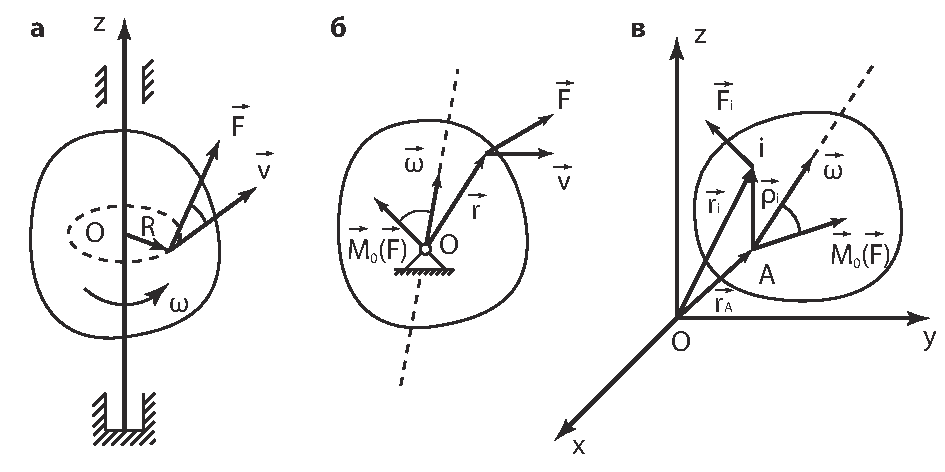
\includegraphics[width=.47\textwidth]{53_01}
    \caption{Рисунки}
    \label{pic53_01}
\end{figure}

При поступательном движении твёрдого тела его можно принять за материальную 
точку и для вычисления работы силы, приложенной к нему, применять все 
формулы для подсчёта элементарной и полной работы силы, приложенной к 
материальной точке.

При вращении твёрдого тела вокруг неподвижной оси скорость точки, где приложена 
сила \( F \) (рис. \ref{pic53_01}а), равна \( v = \omega R \). По формуле
\[ 
	dA = \vec{F}\cdot\vec{v}\,dt = Fv\cos(\hat{Fv})\,dt = 
	F\omega R\cos{\Hat{Fv}}\,dt
\]
Вектор скорости лежит в плоскости, перпендикулярной оси вращения и оси \( Oz \), 
поэтому \( |F\cos\Hat{Fv}| = F_p \), где \( F_p \) -- модуль проекции силы на эту 
плоскость. 

Следовательно, по определению момента силы относительно оси 
\( |M_z| = F_p R\), то есть \( FR\cos\Hat{Fv} = \pm M_z \).

Поэтому элементарную работу силы, приложенной к телу, вращающемуся вокруг 
неподвижной оси, можно выразить так:
\[
	dA = \pm M_z\omega dt = \pm M_zd\phi
\]
где \( d\phi = \omega dt \) -- элементарный угол поворота тела.

Мощность в случае вращения твёрдого тела вокруг неподвижной оси 
вычисляется так:
\[
	N = \frac{dA}{dt} = \pm M_z\omega.
\]

При вращении твёрдого тела вокруг неподвижной точки 
(сферическое движение) (рис. \ref{pic53_01}б) скорость \( v \) точки 
приложения силы \( F \) можно выразить по 
формуле Эйлера, согласно которой \( v = \omega\times r \), где 
\( r \) -- радиус-вектор точки приложения, а \( \omega \) -- 
мгновенная угловая скорость тела. Тогда:
\[ 
	dA = \vec{F}\cdot\vec{v}\,dt = 
	\vec{F}\cdot\left(\vec{\omega}\times\vec{r}\right)\,dt =
	\vec{\omega}\cdot\left(\vec{r}\times\vec{F}\right)\,dt
\]
так как по свойству смешанного произведения векторов 
\( F\cdot\left( \omega\times r\right) = \omega\cdot\left( r\times F\right) \). 
Но \( r\times F = M_0 \) -- момент силы относительно точки или 
центра \( O \). Поэтому 
\[ 
	dA = \vec{\omega}\cdot M_0\,dt = 
	M_0(\vec{F}\cdot\omega\cos(\Hat{\vec{M}_0,\omega})\,dt =
	M_\omega\omega dt = M_\omega\,d\phi,
\]
где \( d\phi \) -- элементарный угол поворота вокруг мгновенной оси 
вращения, а \( M_\omega = M_0\cos\Hat{M_0\omega} \) -- 
проекция вектора \( M_0 \) на направление мгновенной угловой 
скорости, которую называют \emph{моментом силы относительно мгновенной 
оси вращения}.

Мощность силы в этом случае можно выразить так:
\[ 
	N = \frac{dA}{dt} = \vec{M_0}\cdot\vec{\omega} = M_\omega\cdot\omega.
\]

\section{Работа внутренних сил твердого тела + свободное движение}

В самом общем случае (рис. \ref{pic53_01}в), когда на свободное твёрдое тело 
действует система сил \( \left( F_1, F_2, ..., F_n \right) \) скорость 
точки \( v_i \) точки тела с номером \( i \), на которую действет сила 
\( F_i \), можно выразить как 
\( \vec{v_i} = \vec{v}_A + \vec{\omega}\times\vec{\rho_i} \), 
где \( v_A \) -- скорость полюса \( A \), \( \rho_i \) -- радиус-вектор 
точки относительно полюса. Тогда для элементарной работы системы сил 
получим выражение:
\[ 
	dA = \sum_{i=1}^{N} \vec{F}_i
	(\vec{v_a} + \vec{\omega}\times\vec{\rho_i}) =
	\left(\sum_{i=1}^{N}\vec{F}_i\cdot\vec{v}_A\right)\,dt + 
	\sum_{i=1}^{N}\vec{F}_i\cdot(\vec{\omega}\times\vec{\rho_i})\,dt
\]

Воспользовавшись свойствами смешанного произведения векторов, перепишем 
выражение в виде:
\[ 
	dA = \left( \sum_{i=1}^{N}\vec{F}_i \right)\cdot\vec{v}_Adt + 
	\left( \sum_{i=1}^{N} \vec{\rho_i}\times\vec{F}_i\right)\cdot\vec{\omega}dt = 
	\left( \sum_{i=1}^{N}\vec{F}_i \right)\cdot\vec{v}_Adt + 
	\left( \sum_{i=1}^{N} \vec{M}_{Ai} \right)\cdot\vec{\omega}dt
\]

Считая твёрдое тело неизменяемой системой материальных точек, разделим силы, 
действующие на его точки, на внешние и внутренние, то есть 
\( F_i = F^e_i + F^i_i \). Подставляя в предыдущее равенство получаем:
\[ 
	dA = \left( \sum_{i=1}^{N} \vec{F}^e_i \right)\cdot\vec{v}_A\,dt + 
	\left( \sum_{i=1}^{N} \vec{M}_{Ai}^e \right)\cdot\vec{\omega}\,dt +
	\left( \sum_{i=1}^{N} \vec{F}^i_i \right)\cdot\vec{v}_A\,dt + 
	\left( \sum_{i=1}^{N} \vec{M}_{Ai}^i \right)\cdot\vec{\omega}\,dt
\]

В последнем выражении главный вектор и главный момент внутренних сил 
твёрдого тела, согласно свойствам внутренних сил системы, равны нулю:
\[ 
	\sum\vec{F}^i_i = \vec{R}^i = 0;\quad 
	\sum\vec{M}_{Ai}^i = \vec{M}^i_A = 0
\]

Следовательно, \emph{элементарная \( dA^i\) и полная работа \( A^i \), 
а также мощность \( N^i \) внутренних сил абсолютно твёрдого тела 
равна нулю.}

\newpage
